%------------------------ Packages ------------------------
\documentclass[12pt,a4paper]{article}
\usepackage[latin1]{inputenc}
\usepackage[T1]{fontenc}
\usepackage[pdftex]{graphicx}
\usepackage{float}
\usepackage{amsmath}
\usepackage{amssymb}
\usepackage[FIGTOPCAP]{subfigure}
\usepackage{color}
\usepackage[hidelinks]{hyperref}

\newcommand{\version}{\IfFileExists{../../version.txt}
{\input{../../version.txt}}
{\input{../../../version.txt}}
}

\newcommand{\command}[1]{%
\indent \fcolorbox{black}{white}{%
   \begin{minipage}{\dimexpr\textwidth-\parindent\relax}%
      #1
   \end{minipage}%
}
}

\newsavebox{\FVerbBox}
\newenvironment{sample}
{\par \vspace{0.2cm} \begin{lrbox}{\FVerbBox}
\begin{minipage}{\dimexpr\textwidth-\parindent\relax}}
{\end{minipage}
\end{lrbox}
\fcolorbox{black}{lightgray}{\usebox{\FVerbBox}}
\vspace{0.2cm}}

\newenvironment{sampletitle}
{\vspace{0.2cm} \noindent\textbf{Example} :
\begin{sample}}
{\end{sample}}

\newcommand{\samplecomment}[1]{%

\textit{#1}
}

\newcommand{\seealso}[1]{\vspace{0.2cm} \noindent\textbf{See also} :\par #1}

% tikz
\usetikzlibrary{calc}
\usetikzlibrary{arrows}
\usetikzlibrary{shadows}

\tikzset{block/.style={draw, text centered, fill=gray!10,drop shadow}}
\tikzset{connect/.style={draw, line width=1 pt}}

\begin{document}

\begin{center}
\textbf{\huge  \underline{Laplacian operator}}
\end{center}
\vspace{0.5cm}


The Laplacian operator is used for edge detection algorithms. It is a discrete differentiation operator who computes, at each point in the image, an approximation of the horizontal and vertical gradient of the image intensity function.\\


\begin{figure}[h!]
\centering
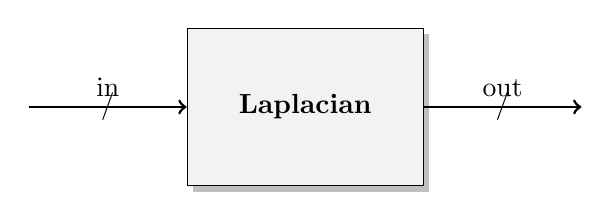
\begin{tikzpicture}
\node[block,rectangle,minimum height=2cm,minimum width=3cm] (bloc) {\textbf{Laplacian}};

\path[connect,<-] ([yshift=0.0cm]bloc.west) -- node{/} node[above]{in} ++(-2cm,0);

\path[connect,->] ([yshift=0.0cm]bloc.east) -- node{/} node[above]{out} ++(2cm,0);
 ([xshift=0.5cm,yshift=-0.6cm]bloc.north);

\end{tikzpicture}
\end{figure}

\vspace{0.5cm}

\begin{figure}[!h]
\centering
\subfigure[Initial image]{
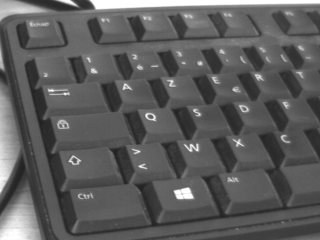
\includegraphics[width=5cm]{laplacian1.png}}
\hspace{2cm}
\subfigure[Image with Laplacian operator]{
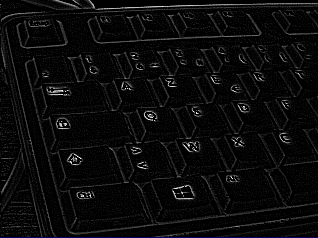
\includegraphics[width=5cm]{laplacian2.png}}
\end{figure}

\section*{Properties}
\properties{
enable & bool & Enable the processing \\ 
weight & matrix & weight of the elements of the Kernel \\
filter\_type & enum & choice between different kernels of the Laplacian \\ 
}

\vspace{0.5cm}

\section*{Constants}

\constants{
LINE\_WIDTH\_MAX & Maximum line size of the image : 1280 pixels  \\ 
CLK\_PROC\_FREQ & Frequency clock of the process \\
IN\_SIZE & Size of the input flow : 1 byte \\
OUT\_SIZE & Size of the output flow : 1 byte  \\
WEIGHT\_SIZE & Size of the Kernel : 1 byte  \\
}

\newpage

\section*{Equivalence}
\subsection*{Matlab}

\lstset{language=Matlab}
\begin{lstlisting}
I; % image matrix 3x3
K = [0 1 0 ; 1 -4 1 ; 0 1 0]; % kernel 3x3
I_laplacian = conv2(I,K); % convolved matrix image 

% LAPLACIAN = edge(I, 'laplacian'); 
	% Edge detection using 
	% Laplacian operator

\end{lstlisting}

\url{https://nl.mathworks.com/help/images/ref/edge.html}


\subsection*{OpenCV}

\lstset{language=C++}
\begin{lstlisting}
void cv::Laplacian	
	(	
	InputArray 	src,
	OutputArray 	dst,
	int 		ddepth,
	int 		ksize = 1,
	double 		scale = 1,
	double 		delta = 0,
	int 		borderType = BORDER_DEFAULT 
)		

\end{lstlisting}

\url{http://docs.opencv.org/}

\section*{Mathematical formalism}

The Laplacian operator is defined as the sum of the second derivatives Laplace expressions and calculated as sum of differences over the nearest neighbours of the central pixel.\\

There are different Laplacian Kernels : 4-connexe, 8-connexe and Robinson kernel.\\

\begin{center}
$
\begin{matrix}
\bigtriangledown_{C4} = \begin{pmatrix}
0 & 1 & 0\\ 
1 & -4 & 1\\ 
0 & 1 & 0
\end{pmatrix} ,\quad  & \bigtriangledown_{C8} = \begin{pmatrix}
1 & 1 & 1\\ 
1 & -8 & 1\\ 
1 & 1 & 1
\end{pmatrix} ,\quad  &
\bigtriangledown_{Rob} = \begin{pmatrix}
1 & -2 & 1\\ 
-2 & 4 & -2\\ 
1 & -2 & 1
\end{pmatrix}  
\end{matrix}
$
\end{center}

\vspace{0.5cm}

Find more informations on the next link :\\

\url{https://en.wikipedia.org/wiki/Discrete_Laplace_operator}

\end{document}